\section{Goldendoor}\label{goldendoor}

Tags: Città Creatore: Lorenzo

\section{Goldendoor}\label{goldendoor-1}

\begin{center}\rule{0.5\linewidth}{0.5pt}\end{center}

Informazioni Generali

\begin{figure}
\centering
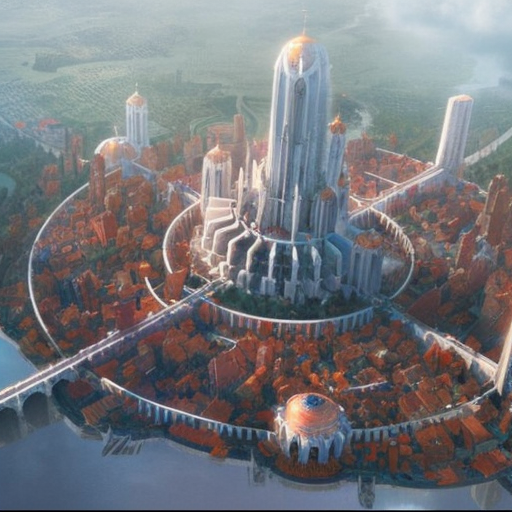
\includegraphics{fantasy-city-trending-on-artstation-sharp-focus-studio-photo-intricate-details-highly-detailed.png}
\caption{fantasy-city-trending-on-artstation-sharp-focus-studio-photo-intricate-details-highly-detailed.png}
\end{figure}

Tipo di Luogo: Capitale

Dimensioni:

Altitudine: 254 m slm

Popolazione: 500 000 abitanti

Paese: Dishartha

Luogo: Maridonia

\begin{center}\rule{0.5\linewidth}{0.5pt}\end{center}

\subsection{1. Descrizione Generale}\label{descrizione-generale}

\begin{center}\rule{0.5\linewidth}{0.5pt}\end{center}

Goldendoor è una città dalle meraviglie architettoniche e dalla bellezza
mozzafiato. Situata nella regione Sud-Occidentale dell'Impero di
Disharta, è una metropoli imponente che brilla di splendore e lusso. Le
strade larghe sono costeggiate da maestosi palazzi nobiliari, l'aria è
pervasa dal profumo dei giardini ben curati e le piazze sono adornate da
fontane scintillanti. Tuttavia, dietro questa facciata di opulenza si
nasconde una realtà ben diversa. La città ospita una popolazione
eterogenea, con una marcata divisione tra i ricchi e i poveri. Un
quartiere malfamato, al di là del fiume, sovraffollato e dominato dalla
malavita, si estende alle ombre delle sontuose dimore nobiliari.

\subsection{2. Storia}\label{storia}

\begin{center}\rule{0.5\linewidth}{0.5pt}\end{center}

Goldendoor ha una storia lunga e complessa. Fondata secoli fa come un
modesto insediamento, la città ha prosperato grazie alle conquiste
militari, diventando in pochi secoli la capitale di uno degli Imperi più
estesi dell'intero pianeta. Nel corso degli anni, i governanti imperiali
hanno investito enormi risorse nella costruzione di palazzi, templi e
opere d'arte per celebrare la grandezza dell'Impero. Tuttavia, questa
opulenza ha portato a una crescente disparità tra le classi sociali, con
i nobili che vivono nell'abbondanza mentre i poveri che lottano per
sopravvivere nei quartieri più malfamati.

\subsection{3. Geografia}\label{geografia}

\begin{center}\rule{0.5\linewidth}{0.5pt}\end{center}

Goldendoor sorge su una vasta pianura bagnata dal fiume Dor. Le strade
della città sono costruite seguendo un piano regolare, con il maestoso
palazzo imperiale che domina il centro.

\subsection{4. Economia}\label{economia}

\begin{center}\rule{0.5\linewidth}{0.5pt}\end{center}

Goldendoor è il fulcro dell'economia dishartiana. Le attività
commerciali, le banche e gli scambi sono fiorenti, sostenuti dalla
vicinanza con la regione di Valtara, che garantisce un flusso costante
di merci. L'agricoltura prospera nelle terre circostanti, come del resto
in gran parte dell'Impero. Tuttavia, l'enorme divario tra ricchi e
poveri è una caratteristica distintiva dell'economia, con i nobili che
controllano la maggior parte delle risorse e della ricchezza.

\subsection{5. Demografia}\label{demografia}

\begin{center}\rule{0.5\linewidth}{0.5pt}\end{center}

La popolazione di Goldendoor è variegata e numerosa, con oltre 500 mila
abitanti. I nobili, le famiglie aristocratiche e i funzionari imperiali
costituiscono una minoranza privilegiata, mentre la maggior parte della
popolazione vive nelle affollate baracche dei quartieri poveri. La
diversità etnica è comune, con rappresentanti di molte regioni
dell'Impero che chiamano Goldendoor casa.

\subsection{6. Governo}\label{governo}

\begin{center}\rule{0.5\linewidth}{0.5pt}\end{center}

Goldendoor è governata e amministrata direttamente dall'imperatore, il
quale ha anche il potere supremo sull'intero Impero di Disharta. Il
governo locale è affidato a una rete di nobili e funzionari imperiali
nominati dall'Imperatore. Tuttavia, il governo centrale spesso ignora i
bisogni dei cittadini comuni, concentrandosi sul mantenimento del potere
e dello status quo. La presenza della malavita nel quartiere dei poveri
è un segno della corruzione che permea la città.
